\documentclass[tikz, border=10pt]{standalone}
\usepackage{cmbright} % Keeps your sans-serif font consistent
\usetikzlibrary{decorations.pathreplacing}

\begin{document}

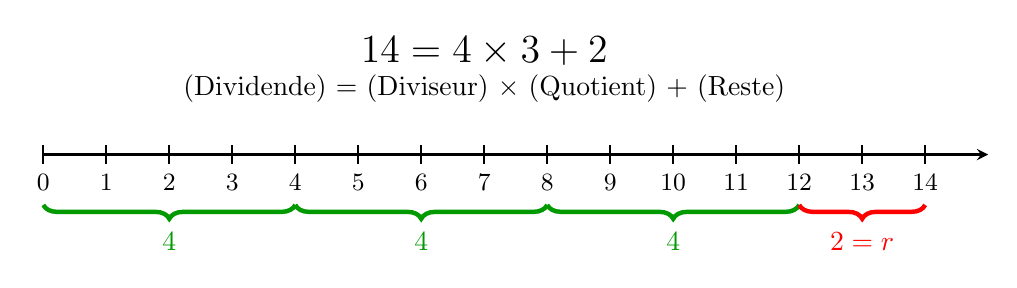
\begin{tikzpicture}[scale=0.8, thick]

    % 1. Draw the main number line (extended to 15 to give some space)
    \draw[->, >=stealth] (0,0) -- (15,0);

    % 2. Draw the 14 uniform marks and numbers using a loop
    \foreach \x in {0,1,...,14} {
        \draw (\x, 0.15) -- (\x, -0.15);
        \node[below] at (\x, -0.15) {\small \x};
    }

    % 3. Draw the quotient groups (3 groups of 4)
    \draw[decorate, decoration={brace, amplitude=5pt, mirror}, green!60!black, ultra thick]
        (0, -0.8) -- (4, -0.8) node[midway, below=6pt] {\(4\)};
        
    \draw[decorate, decoration={brace, amplitude=5pt, mirror}, green!60!black, ultra thick]
        (4, -0.8) -- (8, -0.8) node[midway, below=6pt] {\(4\)};
        
    \draw[decorate, decoration={brace, amplitude=5pt, mirror}, green!60!black, ultra thick]
        (8, -0.8) -- (12, -0.8) node[midway, below=6pt] {\(4\)};

    % 4. Draw the remainder (1 group of 2)
    \draw[decorate, decoration={brace, amplitude=5pt, mirror}, red, ultra thick]
        (12, -0.8) -- (14, -0.8) node[midway, below=6pt] {\(2 = r\)};

    % 5. The Euclidean Division Equation
    \node[above=15pt, align=center] at (7, 0) {
        \Large \(14 = 4 \times 3 + 2\) \\
        \normalsize (Dividende) = (Diviseur) \(\times\) (Quotient) + (Reste)
    };

\end{tikzpicture}

\end{document}